\documentclass[a4paper,10.9pt]{article}
\usepackage[spanish]{babel}
\selectlanguage{spanish}
\usepackage[utf8]{inputenc}
%A Few Useful Packages
\usepackage{marvosym}
\usepackage{fontspec} 					%for loading fonts
\usepackage{xunicode,xltxtra,url,parskip} 	%other packages for formatting
\RequirePackage{color,graphicx}
\usepackage[usenames,dvipsnames]{xcolor}
\usepackage[big]{layaureo} 				%better formatting of the A4 page
% an alternative to Layaureo can be ** \usepackage{fullpage} **
\usepackage{supertabular} 				%for Grades
\usepackage{titlesec}					%custom \section
\usepackage{wrapfig}
\usepackage{parskip} % Remove paragraph indentation
\usepackage{tabularx}
%\usepackage{geometry}


\usepackage{bibentry}
\makeatletter\let\saved@bibitem\@bibitem\makeatother
\usepackage{hyperref}
\makeatletter\let\@bibitem\saved@bibitem\makeatother
%\definecolor{linkcolour}{rgb}{0,0.2,0.6}
%\hypersetup{colorlinks,breaklinks,urlcolor=linkcolour, linkcolor=linkcolour}

%FONTS
\defaultfontfeatures{Mapping=tex-text}
%\setmainfont[SmallCapsFont = Fontin SmallCaps]{Fontin}
%%% modified for Karol Kozioł for ShareLaTeX use
\setmainfont[
SmallCapsFont = Fontin-SmallCaps,
BoldFont = Fontin-Bold,
ItalicFont = Fontin-Italic
]
{Fontin}
%%%



%CV Sections inspired by: 
%http://stefano.italians.nl/archives/26
\titleformat{\section}{\Large\scshape\raggedright}{}{0em}{}[\titlerule]
\titlespacing{\section}{0pt}{3pt}{3pt}
%Tweak a bit the top margin
%\addtolength{\voffset}{-1.3cm}

%Italian hyphenation for the word: ''corporations''
\hyphenation{im-pre-se}

%-------------WATERMARK TEST [**not part of a CV**]---------------
\usepackage[absolute]{textpos}

\setlength{\TPHorizModule}{30mm}
\setlength{\TPVertModule}{\TPHorizModule}
\textblockorigin{2mm}{0.65\paperheight}
\setlength{\parindent}{0pt}


\usepackage{fancyhdr, lastpage}

\pagestyle{fancy}
\renewcommand{\headrulewidth}{0pt}
\fancyhead{}
\fancyfoot{}
\fancyfoot[C]{Página {\thepage} de \pageref{LastPage}}

%--------------------BEGIN DOCUMENT----------------------
\begin{document}

\nobibliography{ref}
  \bibliographystyle{unsrt}

%WATERMARK TEST [**not part of a CV**]---------------
%\font\wm=''Baskerville:color=787878'' at 8pt
%\font\wmweb=''Baskerville:color=FF1493'' at 8pt
%{\wm 
%	\begin{textblock}{1}(0,0)
%		\rotatebox{-90}{\parbox{500mm}{
%			Typeset by Alessandro Plasmati with \XeTeX\  \today\ for 
%			{\wmweb \href{http://www.aleplasmati.comuv.com}{aleplasmati.comuv.com}}
%		}
%	}
%	\end{textblock}
%}



\font\fb=''[cmr10]'' %for use with \LaTeX command

%--------------------TITLE-------------

{ \Huge Martín \textsc{Villegas Pico}}\hfill
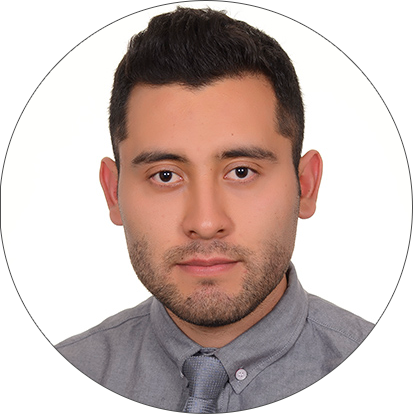
\includegraphics[width=9em]{img/martin.png} \\
\textcolor{black!30}{\rule[.1\baselineskip]{\textwidth}{1pt}}

\begin{center}
%Loja 163 y Unidad Nacional, Urb. La Colina, Sangolquí, Pichincha\\
Ambato, Tungurahua\\
Teléfono: +593 98-346-8911 | Email: \href{mailto:mbvillegas94@gmail.com}{mbvillegas94@gmail.com}
\end{center}


%--------------------SECTIONS-----------------------------------
%Section: Personal Data
%\section{Información Personal}
%
%\begin{tabular}{rl}
    %\textsc{Lugar y fecha de nacimiento:} & Tungurahua, Ecuador  | 19 de abril de 1994\\
    %\textsc{Dirección:}   & Loja 163 y Unidad Nacional, Urb. La Colina, Sangolquí, Pichincha \\
    %\textsc{Teléfono:}     & +593 99-410-1810\\
    %\textsc{Email:}     & \href{mailto:mbvillegas94@gmail.com}{mbvillegas94@gmail.com}
%\end{tabular}

%Section: Education
\section{Educación}
\begin{tabular}{r|l}	
 \textsc{Ene} 2020&  \textsc{Ingeniero en Eléctronica, Automatización y Control}\\&
 \textbf{Universidad de las Fuerzas Armadas ESPE} | Sangolquí, Pichincha\\
&Senescyt Reg. No. 1079-2020-2169562\\
\\
& Tesis: ``Identificación en Tiempo Real de Pérdida de Vía.'' | \small Director: Wilbert \textsc{Aguilar}, Ph.D\\
\multicolumn{2}{c}{} \\
 \textsc{Jul} 2012 &  \textsc{Bachiller en Física y Matemática}\\&
 \textbf{Juan León Mera “La Salle”} | Ambato, Tungurahua\\
\end{tabular}

%Section: Work Experience at the top
\section{Experiencia laboral}
\begin{tabular}{r|p{11cm}}

\textsc{Feb - May 2021} &\textsc{LibélulaSoft - Cía Ltda.} \\&\emph{Desarrollador de software}\\&\footnotesize{Líder de ramo de productos de AIG México}\\&\footnotesize{Desarrollo web Full-Stack usando PHP con el Framework Yii2, ReactJS y MongoDB }\\
\multicolumn{2}{c}{} \\ 
\textsc{Feb 2020 - Ene 2021} &\emph{Diseñador Web Independiente}\\&\footnotesize{Desarrollo Web Full-Stack usando ReactJS con PHP y NodeJS}
\multicolumn{2}{c}{} \\
\textsc{Ago 2018 - Feb 2019} &\textsc{Centro de Investigación de Aplicaciones Militares (CIAM - CICTE)} \\&\emph{Programador web y desarrollador electrónico}\\&\footnotesize{Diseño e implementación del sistema de ingreso al centro de investigación mediante tarjetas magnéticas.}\\&\footnotesize{Remodelación del sistema eléctrico de los escritorios de computación de la Universidad de las Fuerzas Armadas ESPE.}\\  
%\footnotesize{\emph{Ref.: Cpt. William López, Cel.: +593 99-714-6138}}\\
\multicolumn{2}{c}{} \\
 \textsc{Ene - Mar 2018} &\textsc{Universidad de las Fuerzas Armadas ESPE} | Sangolquí, Pichincha \\&\emph{Ayudante de cátedra}\\&\footnotesize{Impartición de cátedra y conducción de laboratorios prácticos de la asignatura de sistemas digitales.}\\ 
%\footnotesize{\emph{Ref.: Ing. Paola León MSc., Cel.: +593 99-191-9087}}\\
\multicolumn{2}{c}{} \\
 \textsc{Feb - Mar 2015}&\textsc{Capacitaciones Guerrero} | Ambato, Tungurahua \\&\emph{Profesor particular de matemáticas y ciencias}\\&\footnotesize{Capacitación a estudiantes universitarios y de secundaria en las áreas de matemáticas, cálculo diferencial e integral, física, y química.}\\ &
%\footnotesize{\emph{Ref.: Ing. Elsa Guerrero, Cel.: +593 98-689-3333}}\\
\end{tabular}

\newpage
\section{Conferencias y publicaciones}
\begin{enumerate}
	\item \bibentry{lidar}
\end{enumerate}
	



%Section: Scholarships and additional info
\section{Certificados}
\begin{tabular}{r|l}	
 \textsc{Mar} 2017 &  \textsc{Competencia avanzada en el idioma Inglés}\\&
 \textbf{Comisión Fulbright Ecuador} | Quito, Pichincha\\

\end{tabular}

%Section: Languages
\section{Idiomas}
\begin{tabular}{rl}
 \textsc{Español:}&Nativo\\
\textsc{Inglés:}&Avanzado\\
\end{tabular}

\section{Habilidades de programación}
\begin{tabular}{rl}
 Desarrollo Web Front-End:& HTML5, CSS3, JavaScript.\\
 Librerías de JavaScript:& ReactJS\\
 Entornos CSS:& Bootstrap y Tailwind CSS\\
 Desarrollo Web Back-End:& PHP, Python, Java y NodeJS.\\
 General:& C/C++\\
 Bases de datos:& MySQL, PostgreSQL, Microsoft SQL Server y MongoDB\\
 Inteligencia Artificial:&  Tensorflow de Google con Python\\
 Otros:& Pipelines CI/CD, Amazon Web Services, Google Cloud Services
\end{tabular}

\end{document}
